\documentclass[]{article}
\usepackage{lmodern}
\usepackage{amssymb,amsmath}
\usepackage{ifxetex,ifluatex}
\usepackage{fixltx2e} % provides \textsubscript
\ifnum 0\ifxetex 1\fi\ifluatex 1\fi=0 % if pdftex
  \usepackage[T1]{fontenc}
  \usepackage[utf8]{inputenc}
\else % if luatex or xelatex
  \ifxetex
    \usepackage{mathspec}
  \else
    \usepackage{fontspec}
  \fi
  \defaultfontfeatures{Ligatures=TeX,Scale=MatchLowercase}
\fi
% use upquote if available, for straight quotes in verbatim environments
\IfFileExists{upquote.sty}{\usepackage{upquote}}{}
% use microtype if available
\IfFileExists{microtype.sty}{%
\usepackage{microtype}
\UseMicrotypeSet[protrusion]{basicmath} % disable protrusion for tt fonts
}{}
\usepackage[margin=1in]{geometry}
\usepackage{hyperref}
\hypersetup{unicode=true,
            pdftitle={Exploring Heterogeneity (Sales Taxes, 2009-2013)},
            pdfauthor={John Bonney},
            pdfborder={0 0 0},
            breaklinks=true}
\urlstyle{same}  % don't use monospace font for urls
\usepackage{color}
\usepackage{fancyvrb}
\newcommand{\VerbBar}{|}
\newcommand{\VERB}{\Verb[commandchars=\\\{\}]}
\DefineVerbatimEnvironment{Highlighting}{Verbatim}{commandchars=\\\{\}}
% Add ',fontsize=\small' for more characters per line
\usepackage{framed}
\definecolor{shadecolor}{RGB}{248,248,248}
\newenvironment{Shaded}{\begin{snugshade}}{\end{snugshade}}
\newcommand{\KeywordTok}[1]{\textcolor[rgb]{0.13,0.29,0.53}{\textbf{#1}}}
\newcommand{\DataTypeTok}[1]{\textcolor[rgb]{0.13,0.29,0.53}{#1}}
\newcommand{\DecValTok}[1]{\textcolor[rgb]{0.00,0.00,0.81}{#1}}
\newcommand{\BaseNTok}[1]{\textcolor[rgb]{0.00,0.00,0.81}{#1}}
\newcommand{\FloatTok}[1]{\textcolor[rgb]{0.00,0.00,0.81}{#1}}
\newcommand{\ConstantTok}[1]{\textcolor[rgb]{0.00,0.00,0.00}{#1}}
\newcommand{\CharTok}[1]{\textcolor[rgb]{0.31,0.60,0.02}{#1}}
\newcommand{\SpecialCharTok}[1]{\textcolor[rgb]{0.00,0.00,0.00}{#1}}
\newcommand{\StringTok}[1]{\textcolor[rgb]{0.31,0.60,0.02}{#1}}
\newcommand{\VerbatimStringTok}[1]{\textcolor[rgb]{0.31,0.60,0.02}{#1}}
\newcommand{\SpecialStringTok}[1]{\textcolor[rgb]{0.31,0.60,0.02}{#1}}
\newcommand{\ImportTok}[1]{#1}
\newcommand{\CommentTok}[1]{\textcolor[rgb]{0.56,0.35,0.01}{\textit{#1}}}
\newcommand{\DocumentationTok}[1]{\textcolor[rgb]{0.56,0.35,0.01}{\textbf{\textit{#1}}}}
\newcommand{\AnnotationTok}[1]{\textcolor[rgb]{0.56,0.35,0.01}{\textbf{\textit{#1}}}}
\newcommand{\CommentVarTok}[1]{\textcolor[rgb]{0.56,0.35,0.01}{\textbf{\textit{#1}}}}
\newcommand{\OtherTok}[1]{\textcolor[rgb]{0.56,0.35,0.01}{#1}}
\newcommand{\FunctionTok}[1]{\textcolor[rgb]{0.00,0.00,0.00}{#1}}
\newcommand{\VariableTok}[1]{\textcolor[rgb]{0.00,0.00,0.00}{#1}}
\newcommand{\ControlFlowTok}[1]{\textcolor[rgb]{0.13,0.29,0.53}{\textbf{#1}}}
\newcommand{\OperatorTok}[1]{\textcolor[rgb]{0.81,0.36,0.00}{\textbf{#1}}}
\newcommand{\BuiltInTok}[1]{#1}
\newcommand{\ExtensionTok}[1]{#1}
\newcommand{\PreprocessorTok}[1]{\textcolor[rgb]{0.56,0.35,0.01}{\textit{#1}}}
\newcommand{\AttributeTok}[1]{\textcolor[rgb]{0.77,0.63,0.00}{#1}}
\newcommand{\RegionMarkerTok}[1]{#1}
\newcommand{\InformationTok}[1]{\textcolor[rgb]{0.56,0.35,0.01}{\textbf{\textit{#1}}}}
\newcommand{\WarningTok}[1]{\textcolor[rgb]{0.56,0.35,0.01}{\textbf{\textit{#1}}}}
\newcommand{\AlertTok}[1]{\textcolor[rgb]{0.94,0.16,0.16}{#1}}
\newcommand{\ErrorTok}[1]{\textcolor[rgb]{0.64,0.00,0.00}{\textbf{#1}}}
\newcommand{\NormalTok}[1]{#1}
\usepackage{graphicx,grffile}
\makeatletter
\def\maxwidth{\ifdim\Gin@nat@width>\linewidth\linewidth\else\Gin@nat@width\fi}
\def\maxheight{\ifdim\Gin@nat@height>\textheight\textheight\else\Gin@nat@height\fi}
\makeatother
% Scale images if necessary, so that they will not overflow the page
% margins by default, and it is still possible to overwrite the defaults
% using explicit options in \includegraphics[width, height, ...]{}
\setkeys{Gin}{width=\maxwidth,height=\maxheight,keepaspectratio}
\IfFileExists{parskip.sty}{%
\usepackage{parskip}
}{% else
\setlength{\parindent}{0pt}
\setlength{\parskip}{6pt plus 2pt minus 1pt}
}
\setlength{\emergencystretch}{3em}  % prevent overfull lines
\providecommand{\tightlist}{%
  \setlength{\itemsep}{0pt}\setlength{\parskip}{0pt}}
\setcounter{secnumdepth}{0}
% Redefines (sub)paragraphs to behave more like sections
\ifx\paragraph\undefined\else
\let\oldparagraph\paragraph
\renewcommand{\paragraph}[1]{\oldparagraph{#1}\mbox{}}
\fi
\ifx\subparagraph\undefined\else
\let\oldsubparagraph\subparagraph
\renewcommand{\subparagraph}[1]{\oldsubparagraph{#1}\mbox{}}
\fi

%%% Use protect on footnotes to avoid problems with footnotes in titles
\let\rmarkdownfootnote\footnote%
\def\footnote{\protect\rmarkdownfootnote}

%%% Change title format to be more compact
\usepackage{titling}

% Create subtitle command for use in maketitle
\newcommand{\subtitle}[1]{
  \posttitle{
    \begin{center}\large#1\end{center}
    }
}

\setlength{\droptitle}{-2em}

  \title{Exploring Heterogeneity (Sales Taxes, 2009-2013)}
    \pretitle{\vspace{\droptitle}\centering\huge}
  \posttitle{\par}
    \author{John Bonney}
    \preauthor{\centering\large\emph}
  \postauthor{\par}
      \predate{\centering\large\emph}
  \postdate{\par}
    \date{January 7, 2019}

\usepackage{booktabs}
\usepackage{longtable}
\usepackage{array}
\usepackage{multirow}
\usepackage[table]{xcolor}
\usepackage{wrapfig}
\usepackage{float}
\usepackage{colortbl}
\usepackage{pdflscape}
\usepackage{tabu}
\usepackage{threeparttable}
\usepackage{threeparttablex}
\usepackage[normalem]{ulem}
\usepackage{makecell}

\usepackage{subfig}

\begin{document}
\maketitle

This document serves as an update to the Dec. 18 version, which focused
on sales tax changes implemented between 2010 and 2012. We now focus on
changes implemented between 2009 and 2013. My comments have been updated
to reflect the changed results.

\subsection{Distribution of Reforms}\label{distribution-of-reforms}

\subsubsection{When are reforms
happening?}\label{when-are-reforms-happening}

\begin{figure}
\centering
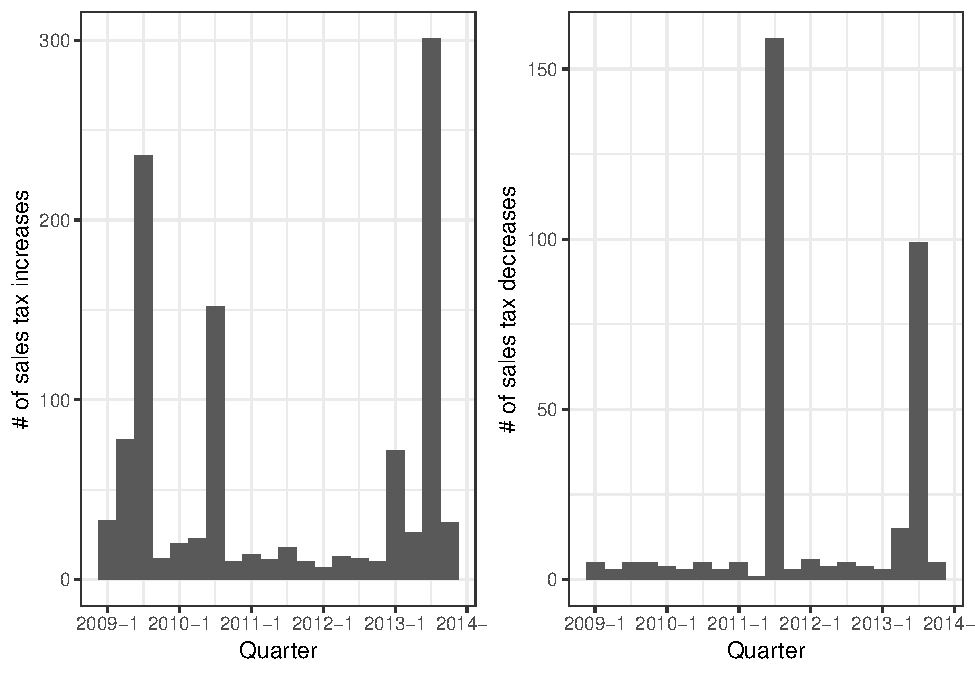
\includegraphics{exploring_heterogeneity_v2_files/figure-latex/plot_distribution-1.pdf}
\caption{\label{fig:plot_dist}Distribution of Sales Tax Changes over
Time}
\end{figure}

As we can see in Figure \ref{fig:plot_dist}, we have five ``spikes'' of
more than 50 sales tax increases occuring in one quarter and two
``spikes'' of similar decreases. Are these spikes individual state-level
reforms, or are they different reforms that happen to coincide?

\begin{Shaded}
\begin{Highlighting}[]
\CommentTok{# Which states are driving the spikes in increases?}

\KeywordTok{with}\NormalTok{(reforms[change }\OperatorTok{==}\StringTok{ "Increase"} \OperatorTok{&}\StringTok{ }\NormalTok{qtr_total_increase }\OperatorTok{>=}\StringTok{ }\DecValTok{50}\NormalTok{],}
     \KeywordTok{table}\NormalTok{(state_name, year_qtr))}
\end{Highlighting}
\end{Shaded}

\begin{verbatim}
##                 year_qtr
## state_name       2009 Q2 2009 Q3 2010 Q3 2013 Q1 2013 Q3
##   Alabama              1       0       0       3       0
##   Arkansas             2       1       0       0      75
##   California          58       1       0      58       0
##   Colorado             0       0       0       2       0
##   Florida              0       0       0       1       0
##   Illinois             0       1       4       0       1
##   Kansas               3       2     105       2       3
##   Louisiana            0       1       1       2       0
##   Massachusetts        0      14       0       0       0
##   Minnesota            0      87       0       0       0
##   Missouri             5       1       3       0       0
##   Nevada               0      17       0       0       0
##   New Mexico           0       7      33       1       2
##   New York             0       1       0       0       0
##   North Carolina       0     100       4       0       0
##   Ohio                 3       0       1       0      88
##   Oklahoma             3       0       0       0       1
##   South Carolina       1       0       0       0       0
##   Tennessee            0       3       0       0       0
##   Virginia             0       0       0       0     131
##   Washington           1       0       1       1       0
##   Wyoming              1       0       0       2       0
\end{verbatim}

The spikes in tax increases appear to be driven by eleven different
state-level reforms (as well as some county-specific reforms in other
states) in Arkansas, California (twice), Kansas, Massachusetts,
Minnesota, Nevada, New Mexico, North Carolina, Ohio, and Virginia.

\begin{Shaded}
\begin{Highlighting}[]
\CommentTok{# Which states are driving the spike in decreases?}

\KeywordTok{with}\NormalTok{(reforms[change }\OperatorTok{==}\StringTok{ "Decrease"} \OperatorTok{&}\StringTok{ }\NormalTok{qtr_total_decrease }\OperatorTok{>=}\StringTok{ }\DecValTok{50}\NormalTok{],}
     \KeywordTok{table}\NormalTok{(state_name, year_qtr))}
\end{Highlighting}
\end{Shaded}

\begin{verbatim}
##                 year_qtr
## state_name       2011 Q3 2013 Q3
##   California          58       0
##   Kansas               0      98
##   North Carolina     100       0
##   Ohio                 1       0
##   Wyoming              0       1
\end{verbatim}

The spikes in tax decreases were specifically driven by three reforms:

\begin{itemize}
\tightlist
\item
  In July 2011, North Carolina \textbf{decreased} its state sales tax by
  1.0\%, from 5.75\% to 4.75\% \emph{(100 counties)}
\item
  In July 2011, California \textbf{decreased} its state sales tax by
  1.0\%, from 8.25\% to 7.25\% \emph{(58 counties)}
\item
  In July 2013, Kansas \textbf{decreased} its state sales tax by 0.15\%,
  from 6.3\% to 6.15\% \emph{(105 counties)}
\end{itemize}

Note that North Carolina and California had increased sales taxes in
2009 and Kansas had increased sales taxes in 2010 (all three of these
increases were by 1.0\%). Consequently, these decreases aren't abrupt
changes in a long-standing policy, but rather a full or partial reversal
of a recent policy change.

\subsubsection{Where are reforms
happening?}\label{where-are-reforms-happening}

\begin{figure}
\centering
\includegraphics{C:/Users/tax_compr_2009-2013.png}
\caption{\label{fig:map}Geographical Distribution of Sales Tax Changes}
\end{figure}

The only state-wide tax changes that appear in this map (Figure
\ref{fig:map}) but are not captured in the previous analysis are:

\begin{itemize}
\tightlist
\item
  Arizona's June 2010 reform, which \textbf{increased} state sales tax
  by 1\%, from 5.6\% to 6.6\%
\item
  Arizona's June 2013 reform, which \textbf{decreased} state sales tax
  by 1\%, from 6.6\% to 5.6\%
\item
  Connecticut's July 2011 reform, which \textbf{increased} state sales
  tax by 0.35\%, from 6.0\% to 6.35\%
\item
  Maine's October 2013 reform, which \textbf{increased} state sales tax
  by 0.5\%, from 5.0\% to 5.5\%
\end{itemize}

\begin{table}

\caption{\label{tab:table_state_changes}Number of counties that increased/decreased sales taxes between 2009 and 2013 (by state)}
\centering
\begin{tabular}[t]{lrrr}
\toprule
State & \# ever increase & \# ever decrease & Total\\
\midrule
Alabama & 11 & 1 & 67\\
Alaska & 0 & 0 & 29\\
Arizona & 15 & 15 & 15\\
Arkansas & 75 & 8 & 75\\
California & 58 & 58 & 58\\
\addlinespace
Colorado & 6 & 3 & 64\\
Connecticut & 8 & 0 & 8\\
Delaware & 0 & 0 & 3\\
Florida & 6 & 5 & 67\\
Georgia & 0 & 0 & 159\\
\addlinespace
Hawaii & 0 & 0 & 5\\
Idaho & 0 & 0 & 44\\
Illinois & 20 & 2 & 102\\
Indiana & 0 & 0 & 92\\
Iowa & 0 & 0 & 99\\
\addlinespace
Kansas & 105 & 100 & 105\\
Kentucky & 0 & 0 & 120\\
Louisiana & 13 & 0 & 64\\
Maine & 16 & 0 & 16\\
Maryland & 0 & 0 & 24\\
\addlinespace
Massachusetts & 14 & 0 & 14\\
Michigan & 0 & 0 & 83\\
Minnesota & 87 & 0 & 87\\
Mississippi & 0 & 0 & 82\\
Missouri & 36 & 5 & 115\\
\addlinespace
Montana & 0 & 0 & 56\\
Nebraska & 0 & 0 & 93\\
Nevada & 17 & 0 & 17\\
New Hampshire & 0 & 0 & 10\\
New Jersey & 0 & 0 & 21\\
\addlinespace
New Mexico & 33 & 5 & 33\\
New York & 5 & 2 & 62\\
North Carolina & 100 & 100 & 100\\
North Dakota & 2 & 1 & 53\\
Ohio & 88 & 6 & 88\\
\addlinespace
Oklahoma & 30 & 8 & 77\\
Oregon & 0 & 0 & 36\\
Pennsylvania & 1 & 0 & 67\\
Rhode Island & 0 & 0 & 5\\
South Carolina & 2 & 0 & 46\\
\addlinespace
South Dakota & 0 & 0 & 66\\
Tennessee & 6 & 0 & 95\\
Texas & 0 & 0 & 254\\
Utah & 1 & 1 & 29\\
Vermont & 0 & 0 & 14\\
\addlinespace
Virginia & 131 & 0 & 133\\
Washington & 6 & 1 & 39\\
West Virginia & 0 & 0 & 55\\
Wisconsin & 2 & 0 & 72\\
Wyoming & 11 & 9 & 23\\
\bottomrule
\end{tabular}
\end{table}

I show a breakdown of all county-level changes, state-by-state, in Table
1.

\subsection{County characteristics}\label{county-characteristics}

Using home price data from Zillow.com and Local Area Unemployment
Statistics obtained from the Bureau of Labor Statistics, we can compare
what happens around the time of the sales tax change in counties that do
and do not change their sales tax rates.

\includegraphics{C:/Users/figs/unemp_ct.png}
\includegraphics{C:/Users/figs/unemp_es.png}
\includegraphics{C:/Users/figs/houseprices_ct.png}
\includegraphics{C:/Users/figs/houseprices_es.png}

\subsubsection{Predictive
characteristics}\label{predictive-characteristics}

We have some variables obtained from Zillow.com and IPUMS National
Historical Geographic Information System (NHGIS) in addition to the
Quarterly Census of Employment and Wages (QCEW) and the Local Area
Unemployment Statistics, both from the Bureau of Labor Statistics (see
Table 2). I use these data (restricted to information determined prior
to the tax change) to see which county characteristics ``predict'' sales
tax changes.

\begin{table}

\caption{\label{tab:table_covariates}Summary of variables}
\centering
\begin{threeparttable}
\begin{tabular}[t]{lll}
\toprule
Variable & Source & Description\\
\midrule
$\texttt{SizeRank}$ & Zillow & Rank of county size (by pop.) (Jan. 2006)\\
$\texttt{median\_home\_price}$ & Zillow & Median home price (Jan. 2006)\\
$\texttt{pop}$ & NHGIS & County pop. (2000)\\
$\texttt{pop\_urban}$ & NHGIS & Pop. living in urban areas (2000)\\
$\texttt{pop\_black}$ & NHGIS & Pop. identifying as black (2000)\\
\addlinespace
$\texttt{pop\_over\_65}$ & NHGIS & Pop. over age 65 (2000)\\
$\texttt{pop\_under\_25}$ & NHGIS & Pop. under age 25 (2000)\\
$\texttt{pct\_pop\_no\_college}$ & NHGIS & Pct. pop. without a college degree (2000)\\
$\texttt{pct\_pop\_bachelors}$ & NHGIS & Pct. pop. with bachelor's degree or higher (2000)\\
$\texttt{median\_income}$ & NHGIS & Median income (2000)\\
\addlinespace
$\texttt{total\_housing}$ & NHGIS & Total housing units (2000)\\
$\texttt{owner\_occupied\_housing}$ & NHGIS & Total owner-occupied housing units (2000)\\
$\texttt{annual\_avg\_emplvl}^{\text{*}}$ & QCEW & Establishment employment level (2006)\\
$\texttt{retail\_employment}$ & QCEW & Retail industry employment (2006)\\
$\texttt{total\_establishments}$ & QCEW & Total number of establishments (2006)\\
\addlinespace
$\texttt{retail\_establishments}$ & QCEW & Total number of retail establishments (2006)\\
$\texttt{food\_and\_drugstores\_empshare}$ & QCEW & Fraction of workers in food and drugstores (2006)\\
$\texttt{total\_mean\_wage}$ & QCEW & Mean wage (2006)\\
$\texttt{retail\_mean\_wage}$ & QCEW & Mean wage in retail industry (2006)\\
$\texttt{laborforce}$ & LAUS & Labor force size (2006)\\
\addlinespace
$\texttt{employed}^{\text{*}}$ & LAUS & Total employment level (2006)\\
$\texttt{unemployed}$ & LAUS & Unemployed level (2006)\\
$\texttt{unemp\_rate}$ & LAUS & Unemployment rate (2006)\\
\bottomrule
\end{tabular}
\begin{tablenotes}
\item[*] Note that there are two measures of employment, one from the QCEW and one from the LAUS. This is because the QCEW estimates employment levels using establishment data, but the BLS adjusts these measures from a place-of-work basis to a place-of-residence basis using commutation factors calculated from the ACS. For more information, see the \href{https://www.bls.gov/lau/laumthd.htm}{\underline{BLS estimation methodology}}.
\end{tablenotes}
\end{threeparttable}
\end{table}

I adapted many of the variables in Table 2 to be in percentage or log
terms for comparability across counties. In addition to these variables,
we have industry employment shares for a number of different industries
from the QCEW.

To determine what features are indicative of a future sales tax change,
I run predictive regressions similar to those run by Deshpande and Li
(2018). I estimate three different models for each type of sales tax
reform (increase and decrease). The first model includes
population-specific covariates relating to housing, employment, income,
race, and education. The second model includes industry employment
shares for the county for six specific industries. The third model
combines the covariates from the first two models, and is as follows:

\[
y_{c} = \beta PopChar_{c2000} + \gamma Housing_{c2000,2006} + \delta LaborForce_{c2006} + \kappa EmpShare_{c2006} + \epsilon_{c},
\]

\begin{table}

\caption{\label{tab:table_predictive_res}Predictive Characteristics}
\centering
\begin{threeparttable}
\begin{tabular}[t]{lllllll}
\toprule
\multicolumn{1}{c}{ } & \multicolumn{3}{c}{Ever decrease} & \multicolumn{3}{c}{Ever increase} \\
\cmidrule(l{2pt}r{2pt}){2-4} \cmidrule(l{2pt}r{2pt}){5-7}
Log(pop.) & 0.304*** &  & 0.509*** & 0.022 &  & 0.191**\\
 & (0.117) &  & (0.139) & (0.076) &  & (0.092)\\
Unemp. rate & 0.179*** &  & 0.147** & 0.029 &  & 0.002\\
 & (0.056) &  & (0.068) & (0.044) &  & (0.051)\\
Log(median home price) & 1.509*** &  & 1.471*** & 1.263*** &  & 1.081***\\
\addlinespace
 & (0.222) &  & (0.282) & (0.164) &  & (0.198)\\
Urbanization rate & -0.018*** &  & -0.014* & -0.007* &  & -0.011**\\
 & (0.006) &  & (0.007) & (0.003) &  & (0.004)\\
Pct. black & 0.007 &  & 0.006 & 0.004 &  & -0.001\\
 & (0.007) &  & (0.008) & (0.005) &  & (0.006)\\
\addlinespace
Pct. over 65 & 0.029 &  & -0.044 & 0.016 &  & -0.015\\
 & (0.036) &  & (0.044) & (0.025) &  & (0.03)\\
Pct. under 25 & 0.009 &  & -0.074** & -0.019 &  & -0.048*\\
 & (0.029) &  & (0.037) & (0.021) &  & (0.025)\\
Pct. no college & -0.05*** &  & -0.056*** & -0.016** &  & -0.023**\\
\addlinespace
 & (0.012) &  & (0.015) & (0.008) &  & (0.01)\\
Log(median income) & -3.635*** &  & -4.873*** & -1.822*** &  & -2.385***\\
 & (0.667) &  & (0.856) & (0.471) &  & (0.56)\\
Housing ownership rate & 0.045*** &  & 0.056*** & 0.041*** &  & 0.041***\\
 & (0.013) &  & (0.018) & (0.009) &  & (0.012)\\
\addlinespace
Retail emp. share &  & -0.134*** & -0.119*** &  & -0.053*** & -0.052**\\
 &  & (0.03) & (0.043) &  & (0.019) & (0.026)\\
Construction emp. share &  & 0.057** & 0.096*** &  & 0.006 & -0.001\\
 &  & (0.025) & (0.035) &  & (0.018) & (0.025)\\
Finance/insurance emp. share &  & -0.229*** & -0.407*** &  & -0.142*** & -0.188***\\
\addlinespace
 &  & (0.062) & (0.089) &  & (0.036) & (0.048)\\
Manufacturing emp. share &  & -0.019** & 0.015 &  & -0.009 & -0.001\\
 &  & (0.01) & (0.017) &  & (0.006) & (0.01)\\
Public admin. emp. share &  & 0.055*** & 0.071*** &  & -0.007 & -0.004\\
 &  & (0.018) & (0.025) &  & (0.014) & (0.019)\\
\addlinespace
Real estate emp. share &  & 0.297*** & 0.068 &  & 0.178** & -0.001\\
 &  & (0.097) & (0.17) &  & (0.081) & (0.115)\\
\hline
Obs. & 1343 & 1463 & 1056 & 1639 & 1833 & 1300\\
\bottomrule
\end{tabular}
\begin{tablenotes}
\item \textit{Note: } 
\item *** p<0.01, ** p<0.05, * p<0.1. Percentages and fractions were multiplied by 100, so coefficients represent a 1 pp increase. Estimation is by logistic regression. Increase only counties are excluded from the "ever increase" estimation and vice versa for the "ever decrease" estimation. Standard errors in parentheses.
\end{tablenotes}
\end{threeparttable}
\end{table}

where \(PopChar_{c2000}\) is a vector of population characteristics;
\(Housing_{c2000,2006}\) is a vector of housing characteristics,
including the local median home price in 2006 and the urbanization and
home ownership rates in 2000; \(LaborForce_{c2006}\) is a vector of
local labor force characteristics in 2006; \(EmpShare_{c2006}\) is a
vector of industry employment shares; and \(\epsilon_c\) encapsulates
all other factors impacting any county's decision to change sales taxes.
Note that the first specification excludes \(EmpShare_{c2006}\), while
the second specification excludes all other variables.

Results are found in Table 3. We see that higher populations, higher
unemployment rates, a more educated population, lower incomes, and
higher home prices are associated with a higher likelihood of
\emph{decreasing} sales taxes; a more educated population, lower
incomes, less retail employment, and less manufacturing are associated
with a higher likelihood of \emph{increasing} sales taxes.

Interestingly, when comparing the results between the ``ever decrease''
and ``ever increase'' groups, the signs of the coefficients on a
majority of the predictive characteristics are the same: percent of the
population with no college (negative), log median income (negative), and
finance/insurance employment share (negative). This indicates that these
counties which are increasing or decreasing sales tax rates are
different from the counties that do not change their sales tax rates,
but different in a similar way.

When interpreting these results, it is important to remember that the
states and time periods mentioned in the \textbf{Distribution of
Reforms} section make up a significant portion of the treatment groups,
so some results may be reflecting characteristics of those states or
those time periods that may not be relevant for tax reforms. As a check,
I re-run the regressiosn with dummies for California and North Carolina
(``ever decrease'') and New Mexico and Kansas (``ever increase'').
Coefficients on these dummies are insignificant (z-scores very close to
0). Most of the previously significant factors remain significant;
however, all coefficients exhibit significant shrinkage. These results
are available upon request.

\section{Seasonality}\label{seasonality}

\subsection{Product-specific
seasonality}\label{product-specific-seasonality}

The goal here is to identify which goods exhibit the most seasonality
over time. I do this on the server due to the size of the dataset. I
estimate the following model on the product-store-quarter-year
(\(psqy\)) level:\footnote{For computational purposes, I instead
  residualize out the linear time trend to obtain
  \(\widetilde{y}_{psqy} = y_{psqy} - \gamma_ptime_{t(q,y)}\) and then
  take the mean of \(\widetilde{y}_{psqy}\) over all stores \(s\) and
  years \(y\) for each product-quarter pair to obtain \(\alpha_{qp}.\)
  This is functionally equivalent to what the estimated product-quarter
  fixed effects would be (without an intercept).}
\[ y_{psqy} = \alpha_{qp} + \gamma_ptime_{t(q,y)} + \epsilon_{psqy},\]
where
\[y_{psqy} = \textrm{ln}\left(\frac{sales_{psqy}}{sales_{psQ_12008}}\right),\]
\(\gamma_p\) is a product-specific linear time effect, and
\(\alpha_{qp}\) is a product-quarter fixed effect. I then calculate a
seasonality range for each product,
\[SR_p = \max_{q}(\alpha_{qp})-\min_{q}(\alpha_{qp}).\] \(SR_p\) is then
essentially the product-specific ratio of normalized log sales of the
season with the highest average sales (peak-season) to the season with
the lowest average sales (low-season).\footnote{Consider this measure
  restricted to only one store \(s\) in just one year, \(y=2008.\) See
  that \[\alpha_{qp} = \ln{\frac{sales_{pq}}{sales_{pQ_1}}}.\] Then we
  have \[
  \begin{aligned}
  SR_p &= \max_{q}(\alpha_{qp})-\min_{q}(\alpha_{qp}) \\
  &= \max_{q}\biggl(\ln{\frac{sales_{pq}}{sales_{pQ_1}}}\biggr) - \min_{q}\biggl(\ln{\frac{sales_{pq}}{sales_{pQ_1}}}\biggr) \\
  &= \ln{\left(\frac{\max_q{(sales_{pq}/sales_{pQ_1}})}{\min_q{(sales_{pq}/sales_{pQ_1}})}\right)} \\
  &= \ln{\left(\frac{\max_q{sales_{pq}}}{\min_q{sales_{pq}}}\right)}
  \end{aligned}
  \] We can extend this to an arbitrary number of stores and years
  (assuming a balanced panel for each product). Let \(\bar{q}\) denote
  the quarter that maximizes \(\alpha_{qp},\) let \(\underline{q}\)
  denote the quarter that minimizes \(\alpha_{qp},\) and let \(N_{s,y}\)
  denote the number of store-years in the data. It is simple to show
  that \[
  SR_p = \frac{1}{N_{s,y}}\sum_{s,y}\ln\biggl(\frac{sales_{ps\bar{q}y}}{sales_{ps\underline{q}y}}\biggr),
  \] which is clearly the average over all store-years of the log ratio
  of sales in \(\bar{q}\) to sales in \(\underline{q}.\)} Taking
\(e^{SR_p}\) gives a rough estimate of the actual ratio of peak-season
sales to low-season sales.\footnote{Continuing notation from footnote 4,
  we have
  \[ e^{SR_p} = \biggl(\prod_{s,y}\frac{sales_{ps\bar{q}y}}{sales_{ps\underline{q}y}}\biggr)^{\frac{1}{N_{s,y}}}\]}
We use \(SR_p\) primarily as an index to compare seasonality across
goods.

We can use these resulting \(SR_p\) indicators to examine the
distribution of seasonality within the 265 best-selling products left in
the balanced panel.

\begin{figure}
\centering
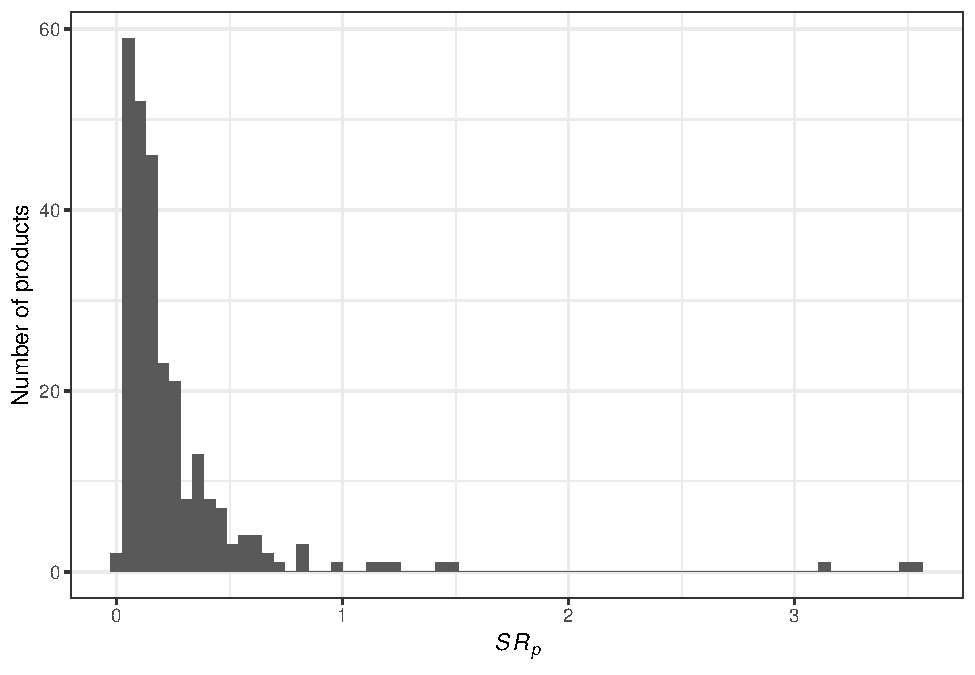
\includegraphics{exploring_heterogeneity_v2_files/figure-latex/plot_seasonality-1.pdf}
\caption{\label{fig:fig3}Distribution of Seasonality Range across
Products}
\end{figure}

Most products appear to exhibit some sort of seasonality (Figure
\ref{fig:fig3}). However, seasonality across products exhibits
considerable heterogeneity, and there are clearly some outliers.

The most seasonal goods by far are specialty chocolates, electric fans,
and sunscreens/sunblocks (see Table 4). Not surprisingly, these are
goods one would expect to be correlated with seasons. Prices of fans and
sun products peak as summer begins, in \(\text{Q}_2,\) and reach their
lowest point as winter begins, in \(\text{Q}_4.\) Specialty chocolates
have highest sales during the quarter that contains Valentine's day.

This serious seasonality is only exhibited for 3 out of the 265 products
we examine, and is thus unlikely to be the driver of seasonality issues
in the data. However, it is worth noting that items with more seasonal
sales seem more likely to be non-food items (and thus taxable), while
items with less seasonal sales are food items.

\begin{table}

\caption{\label{tab:table_seasonality}Products with highest/lowest seasonality range}
\centering
\begin{tabular}[t]{lrrrr}
\toprule
Module description & $SR_p$ & $e^{SR_p}$ & Low season & Peak season\\
\midrule
\addlinespace[0.3em]
\multicolumn{5}{l}{\textbf{Highest $SR_p$}}\\
\hspace{1em}Candy-chocolate-special & 3.56 & 35.15 & 3 & 1\\
\hspace{1em}Fan and ceiling fan appliance & 3.51 & 33.47 & 4 & 2\\
\hspace{1em}Suntan preparations - sunscreens \& sunblocks & 3.13 & 22.84 & 4 & 2\\
\hspace{1em}Charcoal & 1.51 & 4.51 & 4 & 2\\
\hspace{1em}Video and computer games & 1.41 & 4.11 & 2 & 4\\
\hspace{1em}Personal planners binders and folders & 1.22 & 3.40 & 2 & 3\\
\hspace{1em}Fresh strawberries & 1.18 & 3.26 & 4 & 2\\
\hspace{1em}Ice & 1.13 & 3.09 & 1 & 3\\
\hspace{1em}Video products prerecorded & 0.95 & 2.59 & 3 & 4\\
\hspace{1em}Cough syrups \& tablets & 0.84 & 2.32 & 3 & 1\\
\hspace{1em}Frozen meat - ground beef & 0.84 & 2.31 & 4 & 3\\
\hspace{1em}Cameras & 0.82 & 2.27 & 1 & 4\\
\hspace{1em}Candy-chocolate-miniatures & 0.69 & 2.00 & 3 & 4\\
\hspace{1em}Dough products - cookies \& brownies - refrigerated & 0.67 & 1.96 & 2 & 4\\
\hspace{1em}Soup-canned & 0.66 & 1.93 & 2 & 4\\
\addlinespace[0.3em]
\multicolumn{5}{l}{\textbf{Lowest $SR_p$}}\\
\hspace{1em}Dinners-frozen & 0.04 & 1.04 & 4 & 1\\
\hspace{1em}Baby milk and milk flavoring & 0.04 & 1.04 & 3 & 1\\
\hspace{1em}Soap - bar & 0.04 & 1.04 & 1 & 3\\
\hspace{1em}Razor blades & 0.04 & 1.04 & 4 & 3\\
\hspace{1em}Cosmetics-eyebrow \& eye liner & 0.04 & 1.04 & 3 & 4\\
\hspace{1em}Dairy-flavored milk-refrigerated & 0.04 & 1.04 & 2 & 4\\
\hspace{1em}Adult-incontinence & 0.03 & 1.03 & 3 & 1\\
\hspace{1em}Detergents - heavy duty - liquid & 0.03 & 1.03 & 2 & 1\\
\hspace{1em}Detergents-packaged & 0.03 & 1.03 & 4 & 3\\
\hspace{1em}Bakery-muffins-fresh & 0.03 & 1.03 & 4 & 2\\
\hspace{1em}Bakery - bread - fresh & 0.03 & 1.03 & 2 & 3\\
\hspace{1em}Cheese-processed slices-american & 0.03 & 1.03 & 2 & 3\\
\hspace{1em}Bags - tall kitchen & 0.03 & 1.03 & 2 & 1\\
\hspace{1em}Dog food - wet type & 0.02 & 1.02 & 1 & 4\\
\hspace{1em}Tooth cleaners & 0.02 & 1.02 & 4 & 1\\
\bottomrule
\end{tabular}
\end{table}

\subsection{County-specific
seasonality}\label{county-specific-seasonality}

I also estimate county-specific seasonality, using the same method I
used to estimate product-specific seasonality (but replacing
product-level season effects with county-level season effects). Note
that this implicitly weights all store-product level sales equally
within each county and does not account for interactions between product
and county seasonality. I denote the resulting seasonality range
\(SR_c.\)

\begin{figure}
\centering
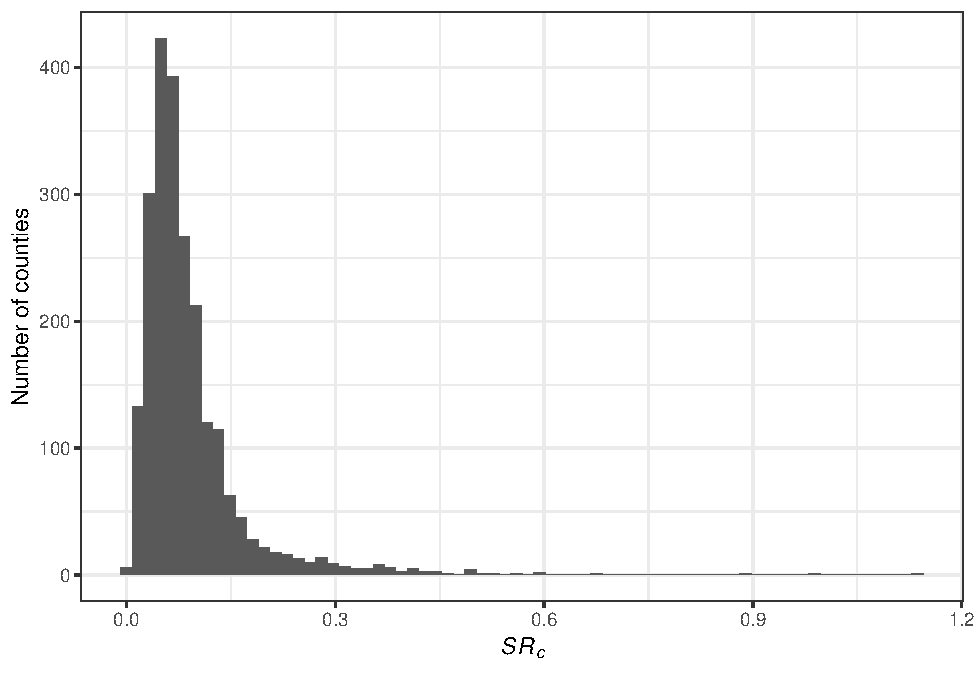
\includegraphics{exploring_heterogeneity_v2_files/figure-latex/plot_seasonality_county-1.pdf}
\caption{\label{fig:fig4}Distribution of Seasonality Range across
Counties}
\end{figure}

We can see in (Figure \ref{fig:fig4}) that county-specific seasonality
follows a similar pattern as product-specific seasonality, but with a
shorter right tail (note the differences in the x-axis scale between
Figure \ref{fig:fig3} and Figure \ref{fig:fig4}). There are some
outliers on the right tail of the distribution.

A t-test shows that the mean populations of counties with \(SR_c < 0.3\)
and those with \(SR_c >= 0.3\) are significantly different (t-stat =
6.1) - counties with abnormally large \(SR_c\) are on average smaller
counties.\footnote{These results hold when population is replaced with
  an ordered population-rank variable (t-stat = -3.5)}

\begin{table}

\caption{\label{tab:table_seasonality_county}Counties with highest/lowest seasonality range}
\centering
\begin{tabular}[t]{lrrrr}
\toprule
County & $SR_p$ & $e^{SR_p}$ & Low season & Peak season\\
\midrule
\addlinespace[0.3em]
\multicolumn{5}{l}{\textbf{Highest $SR_p$}}\\
\hspace{1em}Currituck County NC & 1.14 & 3.13 & 1 & 3\\
\hspace{1em}Cape May County NJ & 0.99 & 2.69 & 1 & 3\\
\hspace{1em}Dare County NC & 0.88 & 2.42 & 1 & 3\\
\hspace{1em}Worcester County MD & 0.68 & 1.97 & 1 & 3\\
\hspace{1em}Mackinac County MI & 0.60 & 1.82 & 1 & 3\\
\hspace{1em}Dickinson County IA & 0.59 & 1.80 & 1 & 3\\
\hspace{1em}Hancock County ME & 0.56 & 1.75 & 1 & 3\\
\hspace{1em}Barnstable County MA & 0.53 & 1.71 & 1 & 3\\
\hspace{1em}Door County WI & 0.51 & 1.67 & 1 & 3\\
\hspace{1em}La Paz County AZ & 0.50 & 1.65 & 3 & 1\\
\hspace{1em}Lincoln County ME & 0.50 & 1.65 & 1 & 3\\
\hspace{1em}Custer County SD & 0.50 & 1.65 & 1 & 3\\
\hspace{1em}Vilas County WI & 0.49 & 1.63 & 1 & 3\\
\hspace{1em}Montmorency County MI & 0.46 & 1.58 & 1 & 3\\
\hspace{1em}Collier County FL & 0.45 & 1.56 & 3 & 1\\
\addlinespace[0.3em]
\multicolumn{5}{l}{\textbf{Lowest $SR_p$}}\\
\hspace{1em}Inyo County CA & 0.15 & 1.16 & 1 & 3\\
\hspace{1em}Nevada County CA & 0.15 & 1.16 & 2 & 3\\
\hspace{1em}Anderson County KS & 0.15 & 1.16 & 3 & 4\\
\hspace{1em}Willacy County TX & 0.15 & 1.16 & 3 & 1\\
\hspace{1em}Erie County OH & 0.15 & 1.16 & 1 & 3\\
\hspace{1em}Wexford County MI & 0.15 & 1.16 & 1 & 3\\
\hspace{1em}Fentress County TN & 0.15 & 1.16 & 2 & 4\\
\hspace{1em}Crittenden County KY & 0.15 & 1.16 & 1 & 4\\
\hspace{1em}Lewis County NY & 0.15 & 1.16 & 2 & 4\\
\hspace{1em}Hughes County SD & 0.15 & 1.16 & 1 & 4\\
\hspace{1em}Modoc County CA & 0.15 & 1.16 & 1 & 3\\
\hspace{1em}Garfield County CO & 0.15 & 1.16 & 1 & 3\\
\hspace{1em}McDonald County MO & 0.15 & 1.16 & 4 & 3\\
\hspace{1em}Larue County KY & 0.15 & 1.16 & 2 & 4\\
\hspace{1em}Barbour County WV & 0.15 & 1.16 & 1 & 3\\
\bottomrule
\end{tabular}
\end{table}


\end{document}
